\documentclass[11pt,a4paper]{article}

\usepackage[utf8]{inputenc}
\usepackage[T1]{fontenc}
\usepackage[margin=2.5cm]{geometry}
\usepackage{amsmath,amssymb,bm}
\usepackage{booktabs}
\usepackage{array}
\usepackage{enumerate}
\usepackage{xcolor}
\usepackage{hyperref}
\usepackage{tikz}

\hypersetup{colorlinks=true, linkcolor=blue, urlcolor=blue}

\newcommand{\points}[1]{\textbf{(#1\,\%)}}
\newcommand{\subpoints}[1]{\textit{(#1\,\%)}}

\title{TMA4268 Statistical Learning V2026\\[0.3em]
\large Mock Exam 2 (estimated final exam)}
\author{Compiled by Claude for Anders Bekkevard\\[0.2em]
\small Based on the Apr 28 exam-review lecture, the 2023--2025 finals, and the prof's stated scope rule}
\date{Mock for: May 18, 2026 (real exam date)}

\begin{document}
\maketitle

\noindent\fbox{\parbox{\dimexpr\textwidth-2\fboxsep-2\fboxrule}{%
\textbf{Instructions.}
\begin{itemize}
  \item \textbf{Duration:} 4 hours. \textbf{Open book.} Permitted aids: ISLP (2nd ed.), one handwritten A5 sheet of notes, calculator.
  \item \textbf{No code required.} Write answers as math, plain English, or pseudocode. Do \emph{not} memorize R/Python package names.
  \item \textbf{Show your work} --- partial credit is generously available, including when calculator slips spoil a numeric answer but the setup is correct.
  \item \textbf{No negative scoring.} Always answer, even when unsure.
  \item \textbf{If a question seems broken or ambiguous}, state the assumption you are making in one short sentence and proceed.
  \item Total: \textbf{100 points = 100\,\%}. Per-problem weights given in parentheses.
\end{itemize}}}

\vspace{0.6em}
\noindent\textbf{Grade boundaries (NTNU \emph{prosentvurderingsmetoden}, advisory):}
A: 89--100\,\% \quad B: 77--88\,\% \quad C: 65--76\,\% \quad D: 53--64\,\% \quad E: 41--52\,\% \quad F: 0--40\,\%.

\vspace{1em}
\hrule
\vspace{1em}

%=========================================================
\section*{Problem 1 \points{10} --- Fill-in-the-blank concepts}
%=========================================================

\noindent Read the passage and pick the best word or short phrase for each blank from the choices in parentheses. Each correct fill is worth $1$\,\%.

\bigskip

In statistical learning we often partition the data into three disjoint pieces: a training set used to fit a candidate model, a \underline{\hspace{2cm}}\,(1) (\emph{validation} / \emph{holdout-of-the-residuals} / \emph{bootstrap} / \emph{oob}) set used to choose between candidate models or tune a hyperparameter, and a test set used to estimate the chosen model's final generalization error. When data are too scarce for a clean three-way split we replace the validation set by \underline{\hspace{2cm}}\,(2) (\emph{cross-validation} / \emph{regularization} / \emph{permutation testing} / \emph{label smoothing}); the most common choice in this course is $k$-fold with $k = 5$ or $10$.

A complementary resampling tool, the \underline{\hspace{2cm}}\,(3) (\emph{bootstrap} / \emph{bagging} / \emph{Bayes rule} / \emph{Markov chain}), draws repeated samples \emph{with replacement} of the same size as the original training set, and uses the empirical sampling distribution of a statistic to estimate its standard error and confidence intervals.

For model selection within the regression module we distinguished discrete and continuous approaches. Best-subset selection considers all $2^p$ subsets of predictors, while \underline{\hspace{2cm}}\,(4) (\emph{forward stepwise} / \emph{lasso shrinkage} / \emph{principal component} / \emph{boosted}) selection performs a greedy search that adds one predictor at a time and is computationally tractable even when $p > n$. Among continuous approaches, ridge regression shrinks coefficients toward zero but never sets them exactly to zero, whereas \underline{\hspace{2cm}}\,(5) (\emph{lasso} / \emph{ridge} / \emph{PCR} / \emph{GAM}) can yield \underline{\hspace{2cm}}\,(6) (\emph{sparse} / \emph{dense} / \emph{orthogonal} / \emph{biased}) coefficient vectors because the geometry of its constraint set has corners on the coordinate axes.

For unsupervised analyses on the same data, dimensionality reduction can be performed by \underline{\hspace{2cm}}\,(7) (\emph{principal component analysis} / \emph{ridge regression} / \emph{the bootstrap} / \emph{the F-test}), which finds orthogonal directions of maximal variance. Clustering can be done by $K$-means (which always returns a flat partition into $K$ clusters and can converge to a \underline{\hspace{2cm}}\,(8) (\emph{local} / \emph{global} / \emph{Bayes-optimal} / \emph{deterministic}) minimum depending on initialization) or by hierarchical clustering, which produces a tree-structured nested family of clusterings called a \underline{\hspace{2cm}}\,(9) (\emph{dendrogram} / \emph{biplot} / \emph{scree plot} / \emph{ROC curve}).

In ensemble methods for trees, \underline{\hspace{2cm}}\,(10) (\emph{boosting} / \emph{bagging} / \emph{random forests} / \emph{stacking}) builds many trees \emph{sequentially}, each one trained on residuals (or, more generally, negative gradients) of the running ensemble, and combines them with a small shrinkage factor.

\vfill\eject

%=========================================================
\section*{Problem 2 \points{28} --- Multiple choice, true/false, and short numeric}
%=========================================================

For each subproblem, write \emph{True} or \emph{False} for each statement (or the requested numeric answer). You may add a one-sentence justification but only if you think it helps; do not write essays.

\subsection*{a) The bootstrap \subpoints{3}}
Mark each statement true or false.
\begin{enumerate}[(i)]
  \item Bootstrap samples are drawn from the training data \emph{with} replacement, and each bootstrap sample has the same size $n$ as the original.
  \item A single bootstrap resample is enough to obtain a reasonable estimate of the standard error of a statistic; the role of the number of resamples $B$ is purely computational.
  \item For large $n$, the probability that a given training observation does \emph{not} appear in a particular bootstrap sample approaches $1/e \approx 0.368$.
  \item A common bootstrap-based $95\%$ confidence interval for a scalar statistic $\hat\theta$ is the \emph{percentile interval}: report the $2.5\%$ and $97.5\%$ quantiles of the bootstrap distribution $\{\hat\theta^*_1, \dots, \hat\theta^*_B\}$.
\end{enumerate}

\subsection*{b) Cross-validation and its pitfalls \subpoints{3}}
Mark each statement true or false.
\begin{enumerate}[(i)]
  \item Compared with leave-one-out CV (LOOCV), $5$- or $10$-fold CV typically has lower \emph{variance} as an estimator of the test error, at the cost of a small additional bias.
  \item Suppose you first rank all $p$ predictors by their marginal correlation with $y$ on the \emph{full} training data, keep the top $20$, and then run $10$-fold CV on a logistic regression fit using just those $20$. The resulting CV error is an unbiased estimate of the test error of the procedure.
  \item For ordinary $k$-fold CV to give a sensible estimate of the test error, the observations must be (at least approximately) independent and identically distributed. With strong time-series autocorrelation, naive $k$-fold CV is misleading.
  \item In nested cross-validation, the \emph{outer} folds are used for model selection (hyperparameter tuning) and the \emph{inner} folds for performance assessment.
\end{enumerate}

\subsection*{c) Subset selection \subpoints{3}}
\begin{enumerate}[(i)]
  \item \subpoints{1} How many distinct candidate models does \emph{best-subset selection} fit on $p = 8$ predictors (counting the null model)? \emph{One numeric answer.}
  \item \subpoints{1} How many distinct candidate models does \emph{forward stepwise selection} fit on $p = 8$ predictors (counting the null model)? \emph{One numeric answer.}
  \item \subpoints{1} True or false, with one short justification: ``Backward stepwise selection can be applied in the high-dimensional regime $p > n$.''
\end{enumerate}

\subsection*{d) Cubic and natural splines: counting degrees of freedom \subpoints{3}}
A predictor $x$ is modeled by a piecewise polynomial fit on top of an intercept.
\begin{enumerate}[(i)]
  \item \subpoints{1} A \emph{cubic regression spline} with $K = 5$ interior knots is fit using the truncated-power basis. How many coefficients does the spline term consume (\emph{not} including the global intercept of the model)?
  \item \subpoints{1} A \emph{natural} cubic spline with $K = 5$ interior knots is fit on the same predictor. How many coefficients does the spline term consume (not including the global intercept)?
  \item \subpoints{1} True or false: ``A cubic spline at every knot is continuous in value, in first derivative, and in second derivative; only the third derivative is allowed to jump.''
\end{enumerate}

\subsection*{e) Logistic regression: odds, log-odds, probability \subpoints{3}}
\begin{enumerate}[(i)]
  \item \subpoints{1} A logistic regression on the binary outcome ``heart attack within ten years'' includes a coefficient $\hat\beta_{\text{age}} = 0.04$ for \texttt{age} measured in \emph{years}. By what factor do the odds of a heart attack change when comparing two otherwise identical individuals whose ages differ by $10$ years? (One numeric value, rounded to two decimals.)
  \item \subpoints{1} For a particular individual the fitted linear predictor equals $\hat\eta = -0.5$. What is the predicted probability $\hat p$ of a heart attack within ten years? (One numeric value, rounded to two decimals.)
  \item \subpoints{1} True or false: ``A logistic-regression coefficient $\beta_j$ has the interpretation that a one-unit increase in $x_j$ changes the \emph{probability} of $Y = 1$ by approximately $\beta_j$, holding the other predictors fixed.''
\end{enumerate}

\subsection*{f) Confusion matrix interpretation \subpoints{4}}
A binary classifier is applied to a test set of $1500$ patients. Of these, $300$ truly have the disease. At a chosen threshold the confusion matrix is:
\begin{center}\small
\begin{tabular}{c|cc}
 & \textbf{Predicted: disease} & \textbf{Predicted: no disease} \\ \hline
\textbf{Actual: disease}    & 240 & 60 \\
\textbf{Actual: no disease} & 120 & 1080 \\
\end{tabular}
\end{center}

Compute, with two decimals:
\begin{enumerate}[(i)]
  \item \subpoints{1} Overall test \emph{accuracy} of the classifier.
  \item \subpoints{1} \emph{Sensitivity} (true positive rate).
  \item \subpoints{1} \emph{Specificity} (true negative rate).
  \item \subpoints{1} \emph{Precision} (positive predictive value) $= \mathrm{TP}/(\mathrm{TP}+\mathrm{FP})$.
\end{enumerate}

\subsection*{g) $K$-means clustering \subpoints{3}}
Mark each statement true or false.
\begin{enumerate}[(i)]
  \item Given a fixed initialization, the $K$-means algorithm is guaranteed to converge to the \emph{global} minimum of the within-cluster sum of squares.
  \item The within-cluster sum of squares (the $K$-means objective) is \emph{non-increasing} from one iteration to the next.
  \item For predictors measured in very different units (e.g.\ kilograms and meters), running $K$-means on the raw data without standardizing can lead to clusters dominated by the largest-scale variable.
  \item Going from $K = 4$ to $K = 5$ in $K$-means is guaranteed to produce a $5$-cluster solution in which one of the original $4$ clusters is split, with the other three unchanged.
\end{enumerate}

\subsection*{h) Tree ensembles: bagging, random forests, boosting \subpoints{4}}
Mark each statement true or false.
\begin{enumerate}[(i)]
  \item In a random forest, the parameter $m$ (number of predictors sampled per split) controls the correlation between trees: smaller $m$ tends to give \emph{less} correlated trees and therefore more variance reduction.
  \item In bagging and random forests, increasing the number of trees $B$ can eventually cause the ensemble to \emph{overfit} the training data.
  \item In gradient boosting with squared-error loss, fitting the next tree to the current residuals is equivalent to fitting a tree to the \emph{negative gradient} of the loss with respect to the current ensemble's predictions.
  \item Random forests for classification are typically fit with $m \approx \sqrt{p}$, whereas for regression the standard default is $m \approx p/3$.
\end{enumerate}

\subsection*{i) Direction of effect \subpoints{2}}
Mark each statement true or false.
\begin{enumerate}[(i)]
  \item In a smoothing-spline fit, increasing the smoothing parameter $\lambda$ decreases the effective degrees of freedom $\mathrm{tr}(S_\lambda)$ and produces a smoother (less wiggly) fit.
  \item In gradient boosting, decreasing the shrinkage / learning rate $\nu$ \emph{decreases} the number of trees $B$ required to fit the data well; smaller $\nu$ means each tree contributes more, so fewer trees are needed.
\end{enumerate}

\vfill\eject

%=========================================================
\section*{Problem 3 \points{16} --- Theory and hand calculations}
%=========================================================

\subsection*{a) The mathy one: variance of an average of correlated predictors \subpoints{8}}

Let $\hat f^{*1}(x_0), \dots, \hat f^{*B}(x_0)$ be the predictions of $B$ models trained on $B$ different bootstrap samples drawn from the same training set, evaluated at a fixed query point $x_0$. Assume that the $\hat f^{*b}(x_0)$ are identically distributed with common variance
$$\mathrm{Var}\!\left(\hat f^{*b}(x_0)\right) = \sigma^2 \quad \text{for every } b,$$
and pairwise positive correlation
$$\mathrm{Cov}\!\left(\hat f^{*b}(x_0),\, \hat f^{*b'}(x_0)\right) = \rho\,\sigma^2 \quad \text{for every } b \neq b'.$$

Let $\bar f_{\text{bag}}(x_0) = \frac{1}{B}\sum_{b=1}^B \hat f^{*b}(x_0)$ denote the bagged prediction.

\begin{enumerate}[(i)]
  \item \subpoints{4} Show, starting from the definition $\mathrm{Var}(Z) = \mathbb{E}\!\left[(Z - \mathbb{E} Z)^2\right]$ \emph{or} the identity $\mathrm{Var}(\sum_b X_b) = \sum_b \mathrm{Var}(X_b) + \sum_{b\neq b'} \mathrm{Cov}(X_b, X_{b'})$, that
  $$\boxed{\;\mathrm{Var}\!\left(\bar f_{\text{bag}}(x_0)\right) \;=\; \rho\,\sigma^2 \;+\; \frac{1 - \rho}{B}\,\sigma^2.\;}$$
  \item \subpoints{1} What is the limit of $\mathrm{Var}\!\left(\bar f_{\text{bag}}(x_0)\right)$ as $B \to \infty$, holding $\rho$ and $\sigma^2$ fixed?
  \item \subpoints{2} Briefly explain why, in light of (ii), \emph{bagging alone} cannot reduce variance below a positive floor in the typical case where bootstrap-trained trees are highly correlated (for instance because every tree splits on the same dominant predictor at the root). What does the \emph{random forest} algorithm do differently to attack this floor?
  \item \subpoints{1} In what (extreme) special case does the formula above reduce to the familiar $\mathrm{Var}(\bar X) = \sigma^2 / B$?
\end{enumerate}

\subsection*{b) Hierarchical clustering by hand: single linkage \subpoints{5}}
Five observations have the following Euclidean dissimilarity matrix:
$$D = \begin{pmatrix}
0 & 2 & 6 & 10 & 9 \\
2 & 0 & 5 & 9 & 8 \\
6 & 5 & 0 & 4 & 5 \\
10 & 9 & 4 & 0 & 3 \\
9 & 8 & 5 & 3 & 0
\end{pmatrix}.$$

\begin{enumerate}[(i)]
  \item \subpoints{3} Run agglomerative hierarchical clustering with \emph{single} linkage. List \emph{each fusion} and its height, and show the recomputed dissimilarity matrix after \emph{both} of the first two merges.
  \item \subpoints{1} Sketch the resulting dendrogram, labelling the four fusion heights on a properly scaled $y$-axis. The horizontal ordering of the leaves $\{1,2,3,4,5\}$ is not unique --- pick any valid ordering.
  \item \subpoints{1} If you instead used \emph{complete} linkage on the same matrix $D$, would the \emph{first} merge change? Justify in one sentence.
\end{enumerate}

\subsection*{c) The bootstrap, by hand \subpoints{3}}
\begin{enumerate}[(i)]
  \item \subpoints{1} Let $n$ training observations be given. Show that the probability a specific observation $i$ is \emph{not} in a given bootstrap sample equals $(1 - 1/n)^n$. (One line of reasoning is enough.)
  \item \subpoints{1} Evaluate the limit of $(1 - 1/n)^n$ as $n \to \infty$, and state the resulting (approximate) probability that observation $i$ \emph{is} in a given bootstrap sample. (Two numeric values.)
  \item \subpoints{1} You want to estimate the standard error of the sample median $\hat\theta = \mathrm{median}(X_1, \dots, X_n)$, for which no clean closed-form sampling distribution is available. Write down (math or pseudocode is fine) a bootstrap algorithm that returns an estimate $\widehat{\mathrm{SE}}_{\text{boot}}(\hat\theta)$.
\end{enumerate}

\vfill\eject

%=========================================================
\section*{Problem 4 \points{22} --- Data analysis: regression on house prices}
%=========================================================

A statistical-learning class collects a dataset of $n = 506$ neighbourhoods in a metropolitan area. The response variable is the median \texttt{price} of an owner-occupied home (in $1000$ USD). The continuous predictors are:
\begin{itemize}
  \item \texttt{crim} --- per-capita crime rate;
  \item \texttt{rm} --- average number of rooms per dwelling;
  \item \texttt{age} --- proportion of homes built before $1940$ (in \%);
  \item \texttt{dis} --- weighted distance to five employment centres;
  \item \texttt{tax} --- property-tax rate per $10{,}000$ USD;
  \item \texttt{ptratio} --- pupil-teacher ratio in local schools;
\end{itemize}
plus one binary predictor \texttt{chas} (1 if the tract borders a river, 0 otherwise).

The data is split into a training set ($n_\text{train} = 400$) and a test set ($n_\text{test} = 106$). All continuous predictors are standardized to mean $0$, standard deviation $1$ \emph{before} fitting any of the models below.

\subsection*{a) Ordinary least squares with an interaction \subpoints{5}}

The course staff first fits an OLS model with an interaction between \texttt{rm} (rooms) and \texttt{chas} (river dummy):
$$\texttt{price} \;\sim\; \texttt{crim} + \texttt{rm} + \texttt{age} + \texttt{dis} + \texttt{tax} + \texttt{ptratio} + \texttt{chas} + \texttt{rm}\!:\!\texttt{chas}.$$
The output is:

\begin{center}\small
\begin{tabular}{lcccc}
\toprule
 & \textbf{Estimate} & \textbf{Std.\ Error} & \textbf{t-value} & \textbf{Pr($>|t|$)} \\
\midrule
(Intercept)         & $22.50$  & $0.40$   & $56.25$ & $<0.001$ \\
\texttt{crim}       & $-1.20$  & $0.30$   & $-4.00$ & $<0.001$ \\
\texttt{rm}         & $3.80$   & $0.45$   & $8.44$  & $<0.001$ \\
\texttt{age}        & $-0.20$  & $0.35$   & $-0.57$ & $0.569$  \\
\texttt{dis}        & $-1.60$  & $0.45$   & $-3.56$ & $<0.001$ \\
\texttt{tax}        & $-1.10$  & $0.35$   & $-3.14$ & $0.002$  \\
\texttt{ptratio}    & $-1.80$  & $0.30$   & $-6.00$ & $<0.001$ \\
\texttt{chas}       & $1.20$   & $0.85$   & $1.41$  & $0.159$  \\
\texttt{rm:chas}    & $2.00$   & $0.90$   & $2.22$  & $0.027$  \\
\bottomrule
\end{tabular}
\end{center}

\noindent Residual standard error: $4.05$ on $391$ degrees of freedom.\quad
Multiple $R^2 = 0.735$,\ Adjusted $R^2 = 0.730$.

\begin{enumerate}[(i)]
  \item \subpoints{1} How many parameters (counting the intercept) does this model estimate? Verify the count against the printed residual degrees of freedom.
  \item \subpoints{2} A classmate says: ``Being next to the river raises the price by $\hat\beta_{\texttt{chas}} = 1.20$ thousand USD, but the $p$-value is $0.159$, so location on the river is irrelevant.'' Explain in one or two sentences why this reading is wrong \emph{given the interaction in the model}, and write down the implied effect on \texttt{price} of being next to the river for a neighbourhood whose standardized \texttt{rm} equals (a) $0$ and (b) $+1$.
  \item \subpoints{1} Holding the other predictors fixed, by approximately how much does the model predict that \texttt{price} (in thousands of USD) changes for a $1$-standard-deviation increase in \texttt{ptratio}? Compute an approximate $95\%$ confidence interval for this effect, using $1.96$ as the critical value.
  \item \subpoints{1} Briefly say why \texttt{age} ($p = 0.569$) is not by itself sufficient evidence to drop \texttt{age} from the model in this dataset. (One sentence.)
\end{enumerate}

\subsection*{b) Forward stepwise vs.\ best subset \subpoints{3}}
Suppose we instead apply forward stepwise selection on the $p = 7$ \emph{main-effect} predictors (no interactions). At step $4$, the procedure has selected the four predictors $\{\texttt{rm}, \texttt{ptratio}, \texttt{crim}, \texttt{dis}\}$.

\begin{enumerate}[(i)]
  \item \subpoints{1} How many \emph{distinct} candidate models has forward stepwise fit by the time it has chosen its best $4$-predictor model? (Recall: include the null model.)
  \item \subpoints{1} How many distinct candidate models would best-subset selection fit by the time it has chosen its best $4$-predictor model?
  \item \subpoints{1} The course staff observes that, on this dataset, forward stepwise and best subset \emph{disagree} on which $4$-predictor model is best. Give one reason this can happen.
\end{enumerate}

\subsection*{c) Ridge with $10$-fold cross-validation \subpoints{7}}
The same $7$ standardized main-effect predictors are now fed into ridge regression. A $10$-fold cross-validation gives the following CV-MSE profile against $\log \lambda$:

\begin{center}
\begin{tikzpicture}[scale=0.85]
  \draw[->] (0,0) -- (8.3,0) node[right] {$\log\lambda$};
  \draw[->] (0,0) -- (0,6.3) node[above] {CV-MSE};

  \draw[smooth, thick, blue] plot[domain=0.3:7.7] (\x, {2.5 + 0.035*(\x-2.0)*(\x-2.0) + 0.0025*(\x-2.0)*(\x-2.0)*(\x-2.0)});

  \draw[dashed] (2.0,0) -- (2.0,5.6);
  \node[above] at (2.0,5.6) {\small $\hat\lambda_{\min}$};
  \draw[dashed] (3.6,0) -- (3.6,5.6);
  \node[above] at (3.6,5.6) {\small $\hat\lambda_{1\mathrm{SE}}$};

  \foreach \x in {0,2,4,6}
    \draw (\x, 0.06) -- (\x, -0.06) node[below] {\x};
  \foreach \y in {0,1,2,3,4,5,6}
    \draw (-0.06, \y) -- (0.06, \y) node[left,xshift=-0.1cm] {\y};

  \node[blue] at (6.3,4.6) {\small CV curve};
\end{tikzpicture}
\end{center}

\noindent The corresponding test MSEs at the two marked $\lambda$ values, evaluated on the held-out $106$ observations, are:
\begin{center}\small
\begin{tabular}{lcc}
\toprule
 & \textbf{Test MSE} & \textbf{No.\ of nonzero coefficients} \\
\midrule
OLS (full main-effect model, no penalty) & $19.40$ & $7$ \\
Ridge at $\hat\lambda_{\min}$            & $16.20$ & $7$ \\
Ridge at $\hat\lambda_{1\text{SE}}$      & $16.95$ & $7$ \\
\bottomrule
\end{tabular}
\end{center}

\begin{enumerate}[(i)]
  \item \subpoints{1} Write down (math or pseudocode) the objective function that the ridge estimator $\hat\beta^R_\lambda$ minimises for a fixed $\lambda$, being careful about whether the intercept is or is not penalized.
  \item \subpoints{2} Briefly explain why all seven coefficients remain nonzero in the ridge fits at both $\hat\lambda_{\min}$ and $\hat\lambda_{1\text{SE}}$, and contrast with what you would expect from a lasso fit on the same data.
  \item \subpoints{1} Why was it important to \emph{standardize} the predictors before running ridge regression?
  \item \subpoints{2} Compare the test MSE of ridge-at-$\hat\lambda_{\min}$ ($16.20$) to OLS ($19.40$). Interpret in bias--variance terms: what does this tell you about the variance of the OLS estimator on this dataset?
  \item \subpoints{1} Without doing any new computation, would you expect the test MSE of a $7$-predictor \emph{lasso} fit at the lasso CV-optimal $\lambda$ to be \emph{lower}, \emph{higher}, or \emph{comparable} to that of the OLS fit, and why? (Answer in one short sentence; a defensible answer earns full credit.)
\end{enumerate}

\subsection*{d) PCR and spline degrees of freedom \subpoints{4}}

\begin{enumerate}[(i)]
  \item \subpoints{2} The same $7$ standardized predictors are now fed into principal components regression (PCR). The first few principal-component eigenvalues are
  $$\lambda_1 = 2.80,\quad \lambda_2 = 1.60,\quad \lambda_3 = 1.00,\quad \lambda_4 = 0.70,\quad \lambda_5 = 0.40,\quad \lambda_6 = 0.30,\quad \lambda_7 = 0.20.$$
  How many principal components must be retained to explain \emph{at least} $80\%$ of the total variance of the standardized $X$-matrix? Show your calculation.
  \item \subpoints{1} The prof has called principal components regression ``\emph{a discretized version of ridge regression}.'' Briefly explain in what sense both methods place ``pressure'' on the same directions of the predictor space, and what makes PCR ``discrete'' while ridge is ``continuous.''
  \item \subpoints{1} Suppose, instead, you fit a generalized additive model with a \emph{cubic regression spline} on \texttt{rm} with $3$ interior knots, and treat all six remaining continuous predictors linearly. How many degrees of freedom does this GAM consume in total, including the intercept? (Treat \texttt{chas} as a single dummy.)
\end{enumerate}

\subsection*{e) Boosting interpretation \subpoints{3}}

A gradient-boosted tree model with $B = 900$ trees, interaction depth $d = 4$, and shrinkage $\nu = 0.05$ is fit on the same training data. The test MSE comes out to $11.40$, lower than every other method tried above.

\begin{enumerate}[(i)]
  \item \subpoints{1} Explain in one or two sentences what the lower test MSE of boosting (relative to OLS and ridge) suggests about the structure of the relationship between the predictors and \texttt{price}.
  \item \subpoints{1} A junior colleague proposes setting $B = 10{,}000$ ``just to be safe.'' Is this a good idea? Why or why not?
  \item \subpoints{1} You want to recover some interpretability from the boosted ensemble. Name one diagnostic plot and one summary statistic the model can produce that help with this. State, for each, what question it does \emph{and does not} answer.
\end{enumerate}

\vfill\eject

%=========================================================
\section*{Problem 5 \points{24} --- Data analysis: classification of heart disease}
%=========================================================

A clinic records $n = 600$ male patients followed over ten years. The binary response \texttt{chd} (coronary heart disease) equals $1$ if the patient developed CHD during follow-up. Predictors of interest:
\begin{itemize}
  \item \texttt{ldl} --- LDL cholesterol (mmol/L);
  \item \texttt{age} --- in years;
  \item \texttt{sbp} --- systolic blood pressure (mmHg);
  \item \texttt{tobacco} --- cumulative tobacco use (kg);
  \item \texttt{famhist} --- family history (1 = positive, 0 = none);
  \item \texttt{sex} --- in this question we additionally include a small companion subgroup with $\texttt{sex} = 1$ (female) recorded; \texttt{sex} $= 0$ (male) is the reference level.
\end{itemize}

The data is split $400 / 200$ into a training and a test set.

\subsection*{a) Discriminant analysis: LDA vs.\ QDA \subpoints{7}}
You first consider a generative model on a \emph{single} predictor $x = \texttt{ldl}$, with two classes
$Y = 0$ (no CHD) and $Y = 1$ (CHD), and you estimate from the training data:
$$\hat\mu_0 = 4,\qquad \hat\mu_1 = 6,\qquad \hat\sigma^2 = 2,\qquad \hat\pi_0 = 0.5,\qquad \hat\pi_1 = 0.5,$$
under the LDA assumption that the within-class densities are Gaussian with the \emph{shared} variance $\hat\sigma^2$.

\begin{enumerate}[(i)]
  \item \subpoints{2} Write down the two LDA discriminant scores $\delta_0(x)$ and $\delta_1(x)$ as functions of $x$. (Use the formula $\delta_k(x) = x \mu_k/\sigma^2 - \mu_k^2/(2\sigma^2) + \log \pi_k$.)
  \item \subpoints{1} Find the LDA decision boundary by solving $\delta_0(x) = \delta_1(x)$ for $x$. Interpret the answer in one sentence.
  \item \subpoints{1} Suppose now that the priors change to $\hat\pi_0 = 0.8$, $\hat\pi_1 = 0.2$ but all other parameters stay the same. Where does the decision boundary move to? (You may leave $\log 4$ unevaluated, or use $\log 4 \approx 1.386$.) Briefly say (one sentence) why the direction of the shift makes sense.
  \item \subpoints{3} Now relax the shared-variance assumption: assume $\hat\sigma_0^2 = 1$, $\hat\sigma_1^2 = 4$ (so the class-$1$ density is wider), with $\hat\mu_0, \hat\mu_1, \hat\pi_0, \hat\pi_1$ as in the original LDA setting. Write down the corresponding \emph{QDA} discriminant scores
  $$\delta_k(x) = -\frac{x^2}{2\sigma_k^2} + \frac{x\,\mu_k}{\sigma_k^2} - \frac{\mu_k^2}{2\sigma_k^2} - \tfrac{1}{2}\log\sigma_k^2 + \log\pi_k,$$
  and explain in one short sentence why the QDA boundary is \emph{quadratic} in $x$ even though the LDA boundary was linear. (You are not required to solve the QDA boundary equation explicitly.)
\end{enumerate}

\subsection*{b) Logistic regression with an interaction \subpoints{8}}

A logistic regression model is fit on the training set using
$$\text{logit}\bigl(\Pr(\texttt{chd} = 1 \mid X)\bigr)
   \;=\; \beta_0 + \beta_1 \texttt{ldl} + \beta_2 \texttt{age} + \beta_3 \texttt{sex} + \beta_4 (\texttt{age}\!:\!\texttt{sex}) + \beta_5 \texttt{famhist},$$
with $\texttt{sex} = 0$ (male) as the reference. The coefficient table is:

\begin{center}\small
\begin{tabular}{lcccc}
\toprule
 & \textbf{Estimate} & \textbf{Std.\ Error} & \textbf{z-value} & \textbf{Pr($>|z|$)} \\
\midrule
(Intercept)         & $-5.00$ & $0.80$ & $-6.25$ & $<0.001$ \\
\texttt{ldl}        & $0.40$  & $0.10$ & $4.00$  & $<0.001$ \\
\texttt{age}        & $0.06$  & $0.012$ & $5.00$  & $<0.001$ \\
\texttt{sex}        & $1.20$  & $0.90$ & $1.33$  & $0.183$  \\
\texttt{age:sex}    & $-0.04$ & $0.014$ & $-2.86$ & $0.004$  \\
\texttt{famhist}    & $0.80$  & $0.22$ & $3.64$  & $<0.001$ \\
\bottomrule
\end{tabular}
\end{center}

(\texttt{ldl} is in mmol/L; \texttt{age} is in years.)

\begin{enumerate}[(i)]
  \item \subpoints{2} State your encoding assumption for \texttt{sex} explicitly. For each additional year of \texttt{age}, by what factor do the odds of CHD change for (a) a \emph{male} patient and (b) a \emph{female} patient, holding the other predictors fixed? Give both odds-multiplication factors to two decimals.
  \item \subpoints{1} For each additional mmol/L of \texttt{ldl}, by what factor do the odds of CHD change, holding the other predictors fixed? Briefly explain why this factor does \emph{not} depend on \texttt{sex} in the fitted model.
  \item \subpoints{2} Consider a $55$-year-old \emph{male} patient with \texttt{ldl} $= 5$ mmol/L and a positive family history. Compute the linear predictor $\hat\eta$, the fitted probability $\hat p$ of CHD, and the predicted class label at threshold $0.5$.
  \item \subpoints{1} A classmate writes: ``Because $p_{\text{sex}} = 0.183 > 0.05$, the main effect of sex is statistically insignificant, so we can drop the \texttt{sex} term from the model.'' Briefly say why this reasoning is wrong when the model contains an \texttt{age}\!:\!\texttt{sex} interaction.
  \item \subpoints{2} Define, in plain words \emph{appropriate to this CHD setting}, what \emph{sensitivity} and \emph{specificity} mean for this classifier.
\end{enumerate}

\subsection*{c) ROC curve and threshold tuning \subpoints{5}}

At the default threshold $\hat p = 0.5$ the logistic model's test-set confusion matrix is:
\begin{center}\small
\begin{tabular}{c|cc}
 & \textbf{Predicted: chd ($\hat y = 1$)} & \textbf{Predicted: no chd ($\hat y = 0$)} \\ \hline
\textbf{Actual: chd}    & 30   & 50  \\
\textbf{Actual: no chd} & 16   & 104 \\
\end{tabular}
\end{center}

A clinician complains: ``We are missing too many true cases of CHD.'' To explore alternatives, you produce the ROC curve below:
\begin{center}
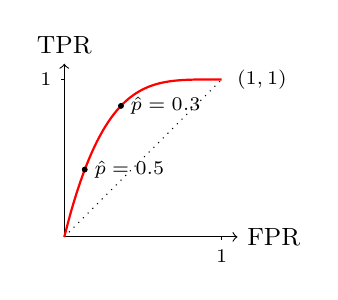
\begin{tikzpicture}[scale=2.0]
  \draw[->] (0,0) -- (1.1,0) node[right] {\small FPR};
  \draw[->] (0,0) -- (0,1.1) node[above] {\small TPR};
  \draw[dotted] (0,0) -- (1,1);
  \draw[smooth, thick, red] plot[domain=0:1] (\x, {1-(1-\x)*(1-\x)*(1-\x)*(1-\x)});
  \draw[fill=black] (0.13, 0.428) circle (0.015) node[right] {\scriptsize $\hat p = 0.5$};
  \draw[fill=black] (0.36, 0.832) circle (0.015) node[right] {\scriptsize $\hat p = 0.3$};
  \node at (1,1) [right=2pt] {\scriptsize $(1,1)$};
  \draw (0,1) -- (-0.02,1) node[left] {\scriptsize 1};
  \draw (1,0) -- (1,-0.02) node[below] {\scriptsize 1};
\end{tikzpicture}
\end{center}

\begin{enumerate}[(i)]
  \item \subpoints{2} From the confusion matrix above, compute the \emph{sensitivity}, \emph{specificity}, and \emph{test error rate} at the threshold $\hat p = 0.5$.
  \item \subpoints{1} Briefly define the \emph{AUC} of the ROC curve and state what AUC $= 0.5$ corresponds to.
  \item \subpoints{2} The clinician proposes lowering the threshold from $0.5$ to $0.3$. Explain (a) how you would expect \emph{sensitivity} and \emph{specificity} to change, and (b) where the operating point moves on the ROC curve. In one short sentence, name a clinical context in which lowering the threshold like this is the right thing to do.
\end{enumerate}

\subsection*{d) A tree-based competitor \subpoints{4}}

You want to fit a tree-based ensemble to compete with the logistic regression. Choose one method and justify your hyperparameter choices.

\begin{enumerate}[(i)]
  \item \subpoints{2} State which tree-based method you would use (e.g.\ bagging, random forest, or gradient boosting). Give a concrete numeric or symbolic value for \emph{each} of its main tuning parameters and justify each choice with one short sentence. ``Sufficiently many trees'' alone is not a sufficient justification; tie the choice to the role the parameter plays.
  \item \subpoints{1} Suppose your chosen method yields, on the same test set, sensitivity $0.50$, specificity $0.85$, and test error rate $0.21$. Compare these to the logistic regression result at threshold $0.5$ from part (c)(i). Which model would you recommend to the clinic, and based on what criterion?
  \item \subpoints{1} The marginal frequency of CHD in this population is approximately $\Pr(\texttt{chd}=1) \approx 0.27$. A trivial classifier that always predicts ``no CHD'' would already achieve a test error rate of about $0.27$. Comment in one or two sentences on whether \emph{test error rate} is the most appropriate metric for choosing between classifiers on this dataset, and what alternative metric or pair of metrics you would privilege.
\end{enumerate}

\vspace{1em}
\hrule
\vspace{0.5em}

\noindent\textbf{End of exam.} \quad Total: $10 + 28 + 16 + 22 + 24 = 100$ points.

\end{document}
